\documentclass[tikz, border=10pt]{standalone}
\usetikzlibrary{positioning, calc, backgrounds, shapes.geometric}

\begin{document}
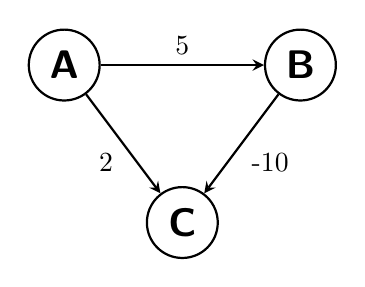
\begin{tikzpicture}[
    vertex/.style={circle, draw, thick, minimum size=0.9cm, inner sep=1pt, font=\sffamily\Large\bfseries},
    directed/.style={->, >=stealth, thick}
]

% Τοποθέτηση Κόμβων (σχηματίζουν τρίγωνο)
\node[vertex] (A) at (0, 2) {A};
\node[vertex] (B) at (3, 2) {B};
\node[vertex] (C) at (1.5, 0) {C};

% Σχεδιασμός Ακμών και Βαρών
\draw[directed] (A) -- node[above] {5} (B);
\draw[directed] (A) -- node[below left] {2} (C);
\draw[directed] (B) -- node[below right] {-10} (C);

\end{tikzpicture}
\end{document}